\chapter{Ausgewählte Technologien}
% languages, libraries, IDEs and tools
\section{Git und GitLab}

\subsection{Versionskontrollsystem}
Oftmals arbeitet ein Entwickler oder ein Entwicklerteam an einem Softwareprojekt, um entweder Fehler zu beheben oder neue Funktionalitäten hinzuzufügen. Hierbei werden Änderungen am Quellcode durchgeführt, die regelmäßig gesichert werden müssen. Diese Änderungen können in manchen Fällen auch dazu führen, dass etwas anderes im Code nicht mehr so funktioniert wie es sollte. Dann werden weitere Änderungen gemacht, um wieder einen lauffähigen Stand herzustellen, jedoch kann es passieren, dass plötzlich gar nichts mehr funktioniert.

\mbox{}\\Abhilfe für dieses Problem bietet ein Versionskontrollsystem, auch als VCS (Version Control System, vlg. \cite{vcs_2019}) bezeichnet , das Änderungen in der Projektentwicklung festhält. Dadurch ist es möglich zu einem späteren beliebigen Zeitpunkt auf ältere Versionen des Systems zurückzugreifen, den aktuellen Code mit früheren Versionen zu vergleichen oder Bugfixes zu implementieren. Arbeiten mehrere Entwickler an denselben Dateien im Quellcode, so kann mitverfolgt werden, welche Person welche Änderungen gemacht hat. Ein Projekt, das mit einem VCS verwaltet wird, heißt Repository. Ein Repository kann als eine Art Datenbank mit allen Änderungen betrachtet werden, die die History repräsentieren. Diese Änderungen sind ein markierter Stand, ein sogenannter Commit, in der Projektentwicklung und werden als Working Copy gespeichert, die einer Kopie des gesamten Projektes entspricht. Ein Commit kann als Schnappschuss oder als kleiner Meilenstein betrachtet werden. Er beinhaltet neben der Working Copy einen Zeitstempel und eine Nachricht, die aussagt, was sich seit dem letzten Commit geändert hat. Die Entwicklungsarbeiten können dabei in mehreren Entwicklungszweigen (engl. Branches) erfolgen. Eine Abspaltung eines Projektes wird hingegen als Fork bezeichnet.

\mbox{}\\Es gibt drei Arten von Version Control Systems:

\begin{itemize}
	\item \textbf{Lokal:} Lokale Versionskontrollsysteme funktionieren nur auf einem Rechner und versionieren eine einzige Datei. Insbesondere in Büroanwendungen kommen Tools wie Revision Control System (RCS) oder Source Code Control System (SCCS) zum Einsatz. Das Dokument speichert  dabei jede Version in seiner eigenen Datei.
	
	\begin{figure}[H]
	\begin{center}
		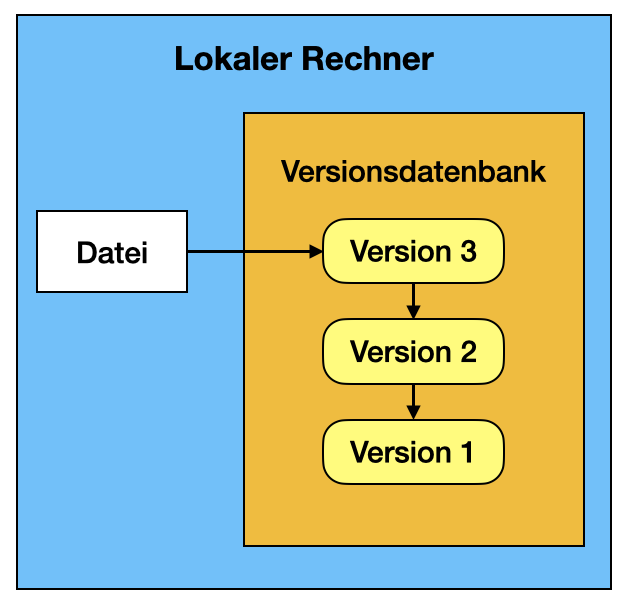
\includegraphics[scale=.65]{images/local_vcs.png}
	\end{center}
		\caption{Lokales Versionskontrollsystem}
	\end{figure}
	
	\item \textbf{Zentral:} Bei einem zentralisierten Versionskontrollsystem gibt es ein Respository, das sich mehrere 		Entwickler in einem Netzwerk miteinander teilen. Es handelt sich hierbei um ein Client-Server-System, das 		von zahlreichen kommerziellen Anbietern verwendet wird. Durch das Concurrent Versions System (CVS) 			wurde dieses Konzept berühmt, aber durch Subversion (SVN) neu implementiert.
	
	\begin{figure}[H]
	\begin{center}
		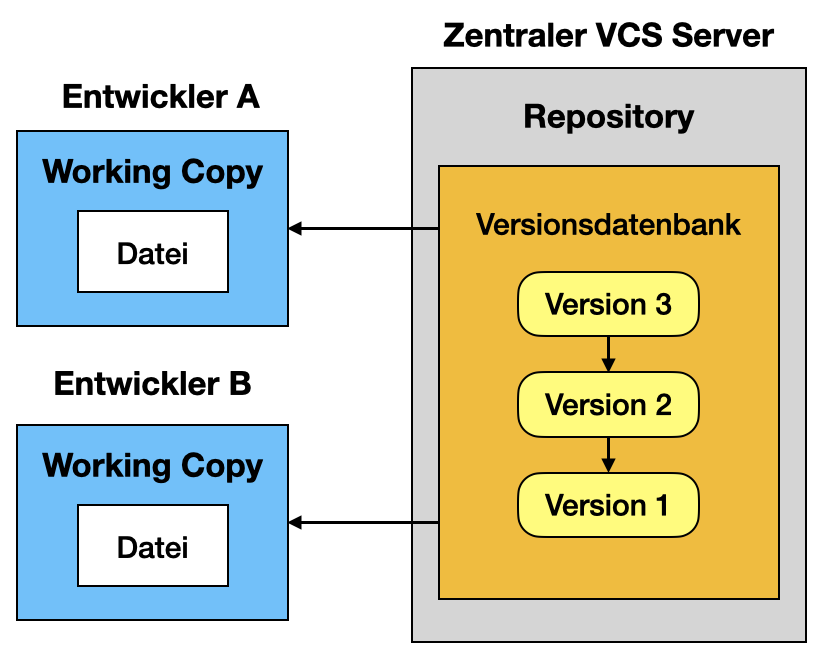
\includegraphics[scale=.65]{images/central_vcs.png}
	\end{center}
		\caption{Zentralisiertes Versionskontrollsystem}
	\end{figure}
	
	\item \textbf{Verteiltes VCS:} Im Gegensatz zum zentralisierten VCS existiert beim verteilten Versionskontrollsystem 		kein zentrales Repository. Jeder am Projekt tätige Entwickler verfügt über ein eigenes Repository, das er mit 		anderen Repositories abgleichen kann. Auch hier ist die History klar ersichtlich. Der einzige Unterschied zu 		den beiden anderen Versionskontrollsystemen ist der, dass Änderungen hier am lokalen Rechner erfolgen 		können. Eine Verbindung mit dem Server ist nicht notwendig.
	
	\begin{figure}[H]
	\begin{center}
		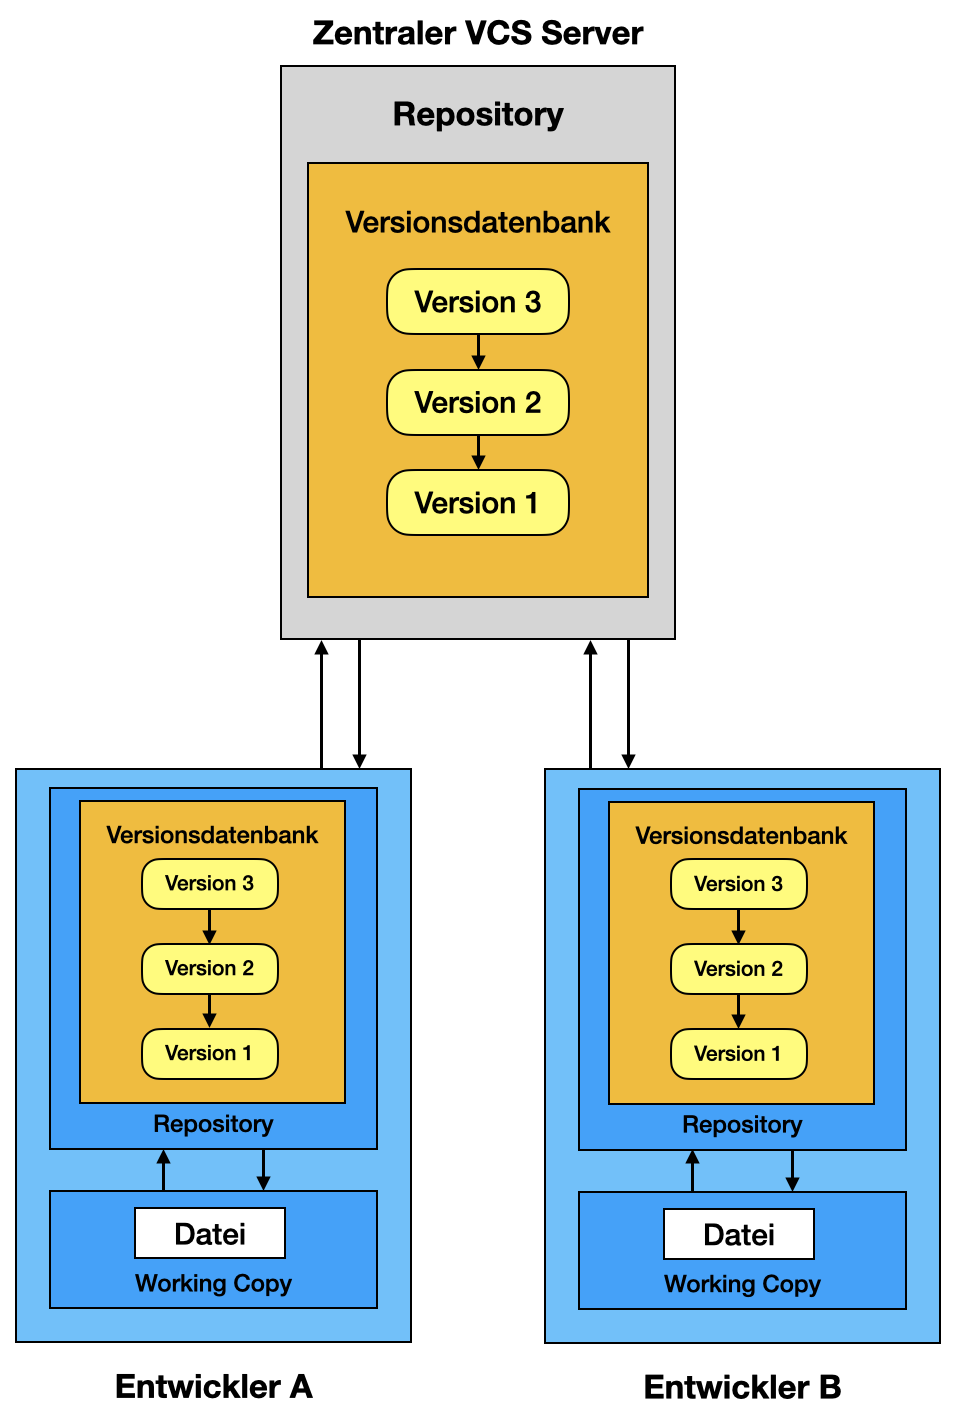
\includegraphics[scale=.6]{images/distributed_vcs.png}
	\end{center}
		\caption{Verteiltes Versionskontrollsystem}
	\end{figure}
\end{itemize}

\subsection{Git}
Git \cite{git_2020} ist ein Open-Source-Tool von Linus Torvalds, dem Entwickler des Betriebssystems Linux, aus dem Jahr 2005. Heutzutage zählt es zu eines der weitverbreitesten Versionsverwaltungssysteme weltweit. Die Softwareentwickler kommen sowohl aus dem kommerziellen als auch aus dem öffentlichen Bereich. Aufgrund seiner Architektur ist Git ein Distributed VCS (DVCS, dt. verteiltes VCS) und funktioniert in zahlreichen Plattformen und Entwicklungsumgebungen. Das bedeutet, dass auf die gesamte History mit allen Entwicklungsarbeiten von jedem Standort aus zugegriffen werden kann. Neben seinem verteilten System ist Git unter anderem auf Performance, Sicherheit und Flexibilität fokussiert.

\subsection{GitLab}

\section{Node.js und npm}

\section{Hypertext Markup Language}

\section{JavaScript}

\section{TypeScript}

\section{Webpack}